\chapter{DMC}

\begin{figure}[h!]
\centering
\subfloat{
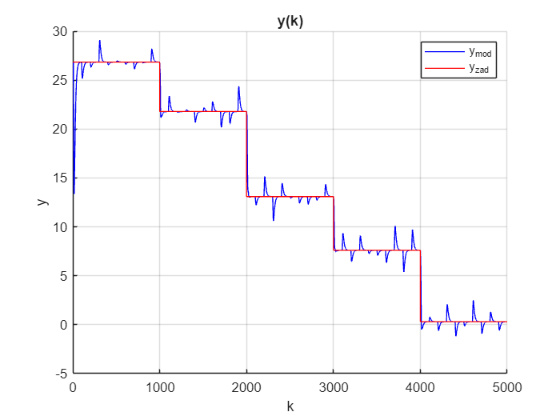
\includegraphics[width=0.8\textwidth]{pictures/dmc_analitic_y_z}}
\hfill
\subfloat{
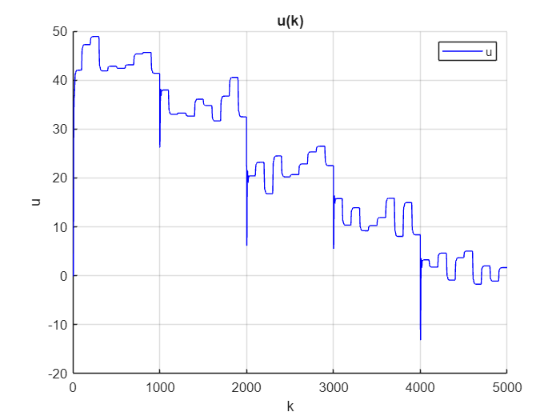
\includegraphics[width=0.8\textwidth]{pictures/dmc_analitic_u_z}}
\caption{Algorytm analityczny DMC bez pomiaru zakłóceń.}
\end{figure}

\newpage

\begin{figure}[h!]
\centering
\subfloat{
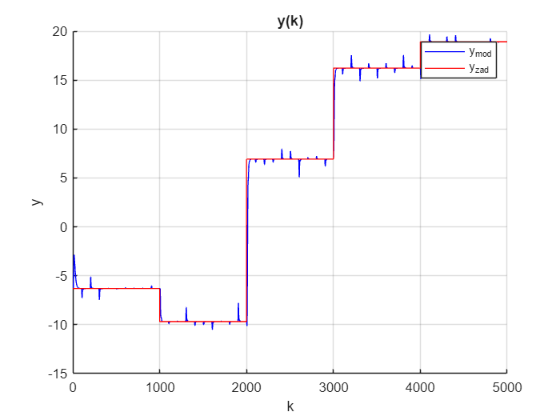
\includegraphics[width=0.8\textwidth]{pictures/dmc_analitic_y}}
\hfill
\subfloat{
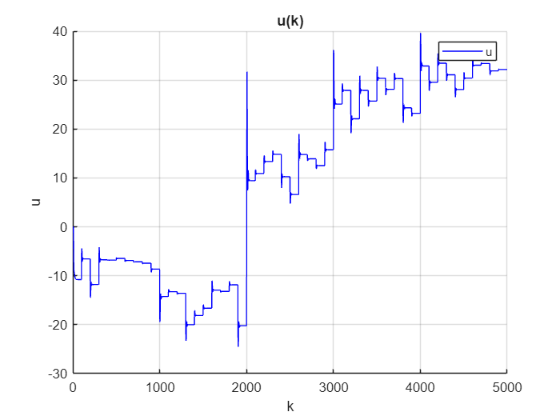
\includegraphics[width=0.8\textwidth]{pictures/dmc_analitic_u}}
\caption{Algorytm analityczny DMC z pomiarem zakłóceń.}
\end{figure}

\newpage

\begin{figure}[h!]
\centering
\subfloat{
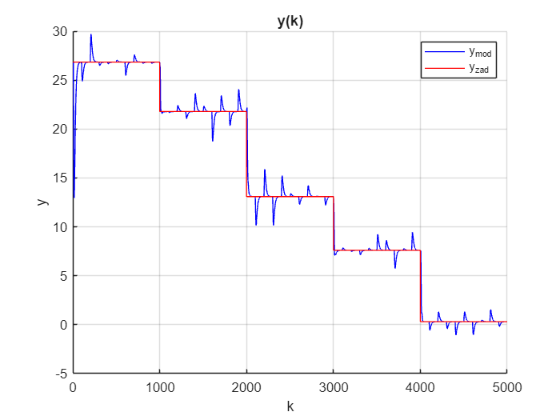
\includegraphics[width=0.8\textwidth]{pictures/dmc_numeric_y_z}}
\hfill
\subfloat{
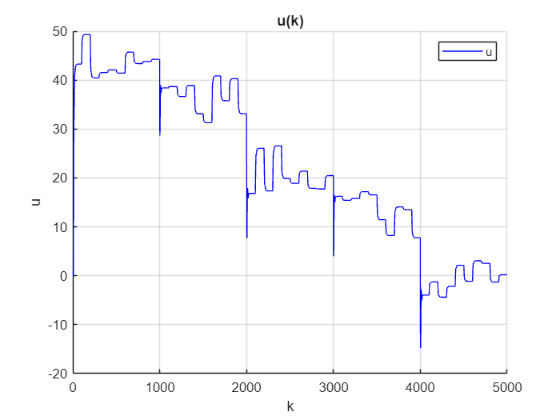
\includegraphics[width=0.8\textwidth]{pictures/dmc_numeric_u_z}}
\caption{Algorytm numeryczny DMC bez pomiaru zakłóceń.}
\end{figure}

\newpage

\begin{figure}[h!]
\centering
\subfloat{
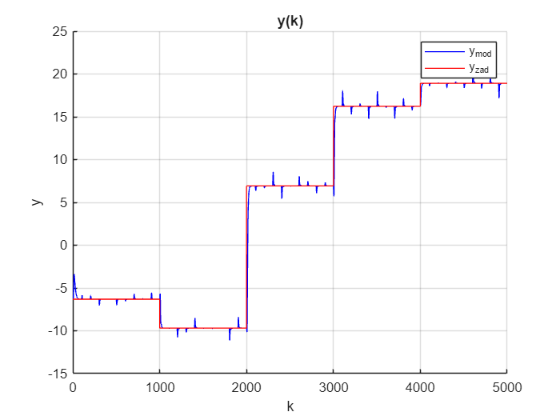
\includegraphics[width=0.8\textwidth]{pictures/dmc_numeric_y}}
\hfill
\subfloat{
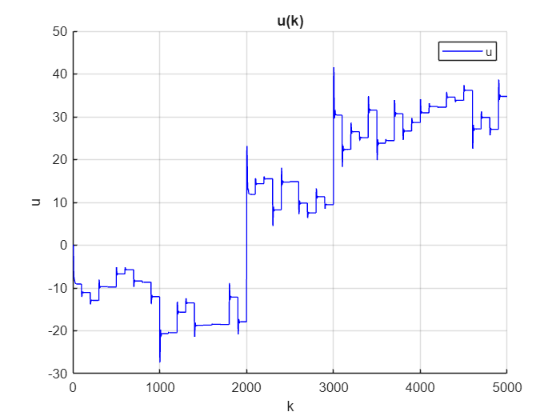
\includegraphics[width=0.8\textwidth]{pictures/dmc_numeric_u}}
\caption{Algorytm numeryczny DMC z pomiarem zakłóceń.}
\end{figure}

Na podstawie przedstawionych przebiegów można wysnuć następujące wnioski:

\begin{itemize}
\item[•] algorytm numeryczny potrafi uwzględnić ograniczenia sygnału sterującego, dzięki temu nie zaobserwowano bardzo dużych przyrostów sterowania
\item[•] pomiar zakłóceń zarówno w wersji analitycznej, jak i numerycznej przynosi bardzo duże korzyści w jakości sterownia 
\end{itemize}